% DSAA2011 Spring 2026 Course Project Report
% Placeholder documentclass — replace with the course-supplied LaTeX style
% file before submission (the project PDF links to it; do not use the
% "preprint" option).
\documentclass[11pt]{article}

\usepackage[margin=1in]{geometry}
\usepackage{graphicx}
\usepackage{booktabs}
\usepackage{subcaption}
\usepackage{hyperref}
\usepackage{amsmath,amssymb}
\usepackage{siunitx}

\graphicspath{{../outputs/}}

\title{Predicting Student Academic Outcomes:\\
A Machine-Learning Pipeline on the Student Dropout Dataset}
\author{Group <GROUP\_ID> \\
  <Member 1>, <Member 2>, <Member 3>, <Member 4>, <Member 5> \\
  DSAA2011, HKUST(GZ), Spring 2026}
\date{May 2026}

\begin{document}
\maketitle

\begin{abstract}
  % 4--6 sentence summary. Fill in once Phase 6 lands.
  We analyse the 4{,}424-row Student Dropout dataset, predicting the
  three-class academic outcome (Dropout / Enrolled / Graduate) from 36
  demographic, academic, and macroeconomic features. A standardised
  preprocessing pipeline, t-SNE visualisation, three clustering
  algorithms, two baseline classifiers, and a validation-driven
  improvement pass constitute the mandatory tasks. Our best baseline
  model is Logistic Regression with test accuracy $0.764$ and
  macro-F1 $0.696$; tuning lifts the Decision Tree's macro AUC from
  $0.73$ to $0.84$. The \emph{Enrolled} class is the hardest across
  every model, consistent with the t-SNE overlap it exhibits with
  the \emph{Graduate} cluster. \textbf{[Phase 6: one sentence on
  open-ended findings.]}
\end{abstract}

% =====================================================================
\section{Introduction}
% Aim: ~0.5 page. Highlight findings and main results up front.

The Student Dropout dataset \cite{uci_dropout} contains 4{,}424
undergraduate records with 36 features covering academic path,
demographics, socio-economic context, and first/second-semester
curricular performance. Our task is to predict the final academic
outcome: Dropout, Enrolled (still enrolled at observation time), or
Graduate. The class distribution is imbalanced
(Graduate $50\%$, Dropout $32\%$, Enrolled $18\%$), which shapes
both our metric choices (macro-F1, macro AUC) and our model
regularisation decisions (\texttt{class\_weight="balanced"}).

Headline results:
\begin{itemize}
  \item Logistic Regression (baseline) reaches test accuracy $0.764$
        and macro-F1 $0.696$, outperforming an unconstrained Decision
        Tree that overfits to $1.000$ train accuracy but only $0.688$
        on test.
  \item t-SNE shows two well-separated clusters (Dropout,
        Graduate) with Enrolled students dispersed between them —
        consistent with confusion-matrix evidence that Enrolled is
        the hardest class.
  \item $K{=}3$ is the preferred cluster count for K-means,
        Hierarchical, and GMM. K-means wins on internal metrics;
        GMM wins on external agreement with true labels; all external
        scores are moderate (Purity $\approx 0.65$).
  \item Validation-driven tuning lifts the Decision Tree's macro AUC
        from $0.729$ to $0.838$, with the binding constraints being
        \texttt{max\_depth=5} and \texttt{class\_weight="balanced"}.
  \item \textbf{[Phase 6 finding: one line on feature engineering /
        additional-model comparison impact.]}
\end{itemize}

% =====================================================================
\section{Mandatory Tasks}

\subsection{Data Preprocessing}
% Aim: ~0.5 page. Methods + observations.

The raw file is semicolon-delimited with no missing values in any of
the 36 columns. We classify features as continuous (19 columns,
e.g.\ \emph{Age at enrollment}, \emph{Unemployment rate}), ordinal
categorical, and nominal categorical (e.g.\ \emph{Marital status},
\emph{Nacionality}, \emph{Mother's occupation}). The preprocessing
pipeline:

\begin{enumerate}
  \item One-hot encode nominal categoricals via
        \texttt{pd.get\_dummies(drop\_first=True)}, expanding $36$
        raw features to $238$ engineered columns.
  \item Standardise the $19$ continuous columns with
        \texttt{StandardScaler} (zero mean, unit variance).
  \item Label-encode the target (Dropout $\to 0$, Enrolled $\to 1$,
        Graduate $\to 2$).
\end{enumerate}

\textbf{Observation:} no explicit missing values, but several nominal
columns (\emph{Mother's qualification}, \emph{Nacionality}) have
long-tailed distributions where specific codes occur fewer than $10$
times. After the $70/30$ stratified split we observe $14$
zero-variance one-hot columns in the training fold; they are
retained (\texttt{StandardScaler} handles them safely) to preserve
the schema across splits.

\subsection{Data Visualisation (t-SNE)}
% Aim: ~0.5 page with figure.

We apply t-SNE (\texttt{sklearn.manifold.TSNE}, perplexity $= 30$,
\texttt{max\_iter} $= 1000$, \texttt{random\_state} $= 42$) to the
preprocessed matrix.

\begin{figure}[h]
  \centering
  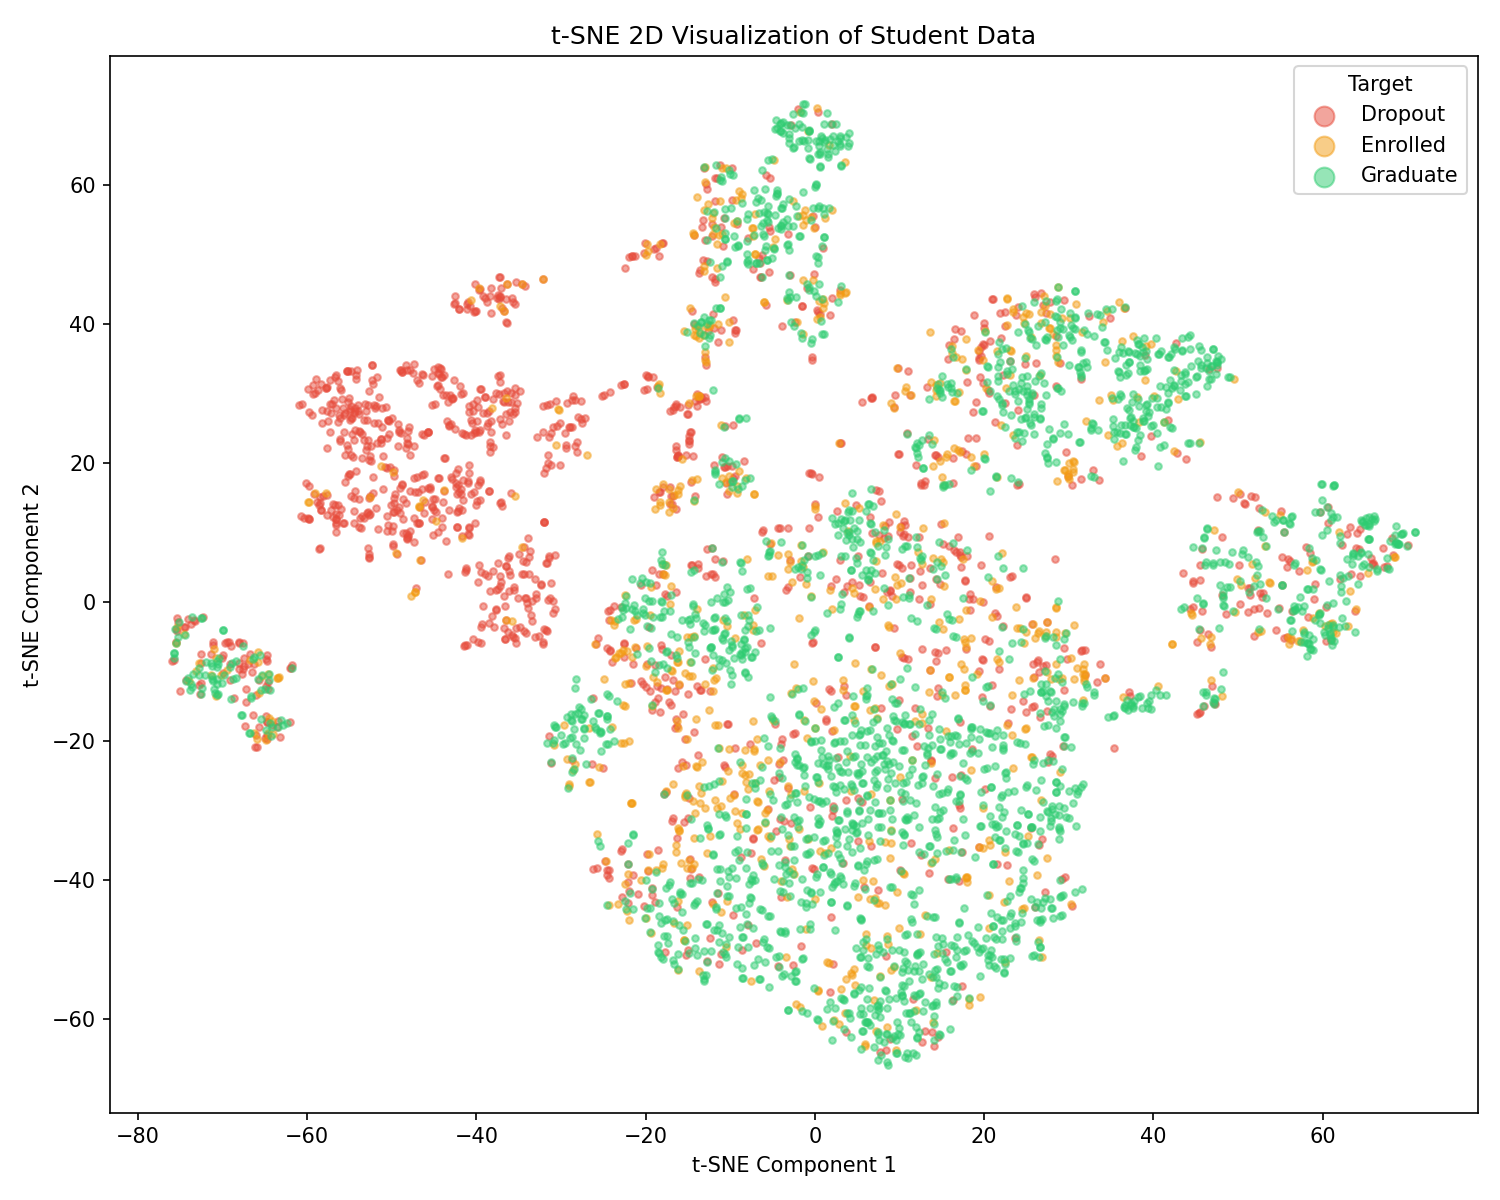
\includegraphics[width=0.65\linewidth]{tsne_2d.png}
  \caption{2D t-SNE projection coloured by true class. Dropout
    (red) and Graduate (green) occupy largely separate regions of the
    embedding; Enrolled (orange) is dispersed, overlapping both.}
  \label{fig:tsne2d}
\end{figure}

A perplexity sweep ($p \in \{5, 15, 30, 50\}$, see
\texttt{outputs/tsne\_perplexity\_comparison.png}) shows the
Dropout/Graduate split is stable, while Enrolled remains diffuse
across every setting --- evidence that its overlap is a real
property of the feature space, not a visualisation artefact.

\subsection{Clustering Analysis}
% Aim: ~1 page. Algorithm descriptions + comparison table + figure.

We compare three algorithms: K-means (distance-based centroids),
Agglomerative Hierarchical Clustering (Ward linkage, bottom-up
merging), and Gaussian Mixture Models (probabilistic, full
covariance). Each is run for $K \in \{2, \ldots, 10\}$; we evaluate
on three internal metrics (Silhouette, Calinski--Harabasz,
Davies--Bouldin) and three external metrics against the true class
labels (ARI, NMI, Purity).

\begin{table}[h]
  \centering
  \caption{Clustering comparison at $K{=}3$. Internal metrics favour
    K-means; external metrics favour GMM; all external scores are
    moderate.}
  \label{tab:cluster}
  \begin{tabular}{lrrrrrr}
    \toprule
    Algorithm    & Silhouette & CH      & DB    & ARI   & NMI   & Purity \\
    \midrule
    K-means      & $0.247$    & $731.45$& $1.73$& $0.162$ & $0.166$ & $0.645$ \\
    Hierarchical & $0.212$    & $645.82$& $1.76$& $0.123$ & $0.134$ & $0.624$ \\
    GMM          & $0.138$    & $472.38$& $2.98$& $0.194$ & $0.166$ & $0.649$ \\
    \bottomrule
  \end{tabular}
\end{table}

\textbf{Best choice:} K-means with $K{=}3$ as the primary method
(best internal separation); GMM as supplementary reference for
probabilistic assignment. The modest external scores indicate that
unsupervised clusters only partially align with academic outcome
labels --- consistent with the t-SNE picture where Enrolled is not
linearly separable.

\subsection{Prediction: Training and Testing}
% Aim: ~1 page. Models + split + confusion matrices + comparison.

\paragraph{Target and models.} We predict the three-class
\texttt{Target} column. Two simple model classes are selected:

\begin{itemize}
  \item \textbf{Decision Tree} (\texttt{DecisionTreeClassifier},
        \texttt{random\_state}$=42$) --- interpretable, handles mixed
        feature types natively, no scaling required.
  \item \textbf{Logistic Regression}
        (\texttt{LogisticRegression}, \texttt{max\_iter}$=1000$) ---
        standard linear baseline for multi-class classification.
        Fitted on \texttt{StandardScaler}-transformed features
        (fit on the training fold only) to avoid numerical overflow
        on the unscaled $238$-column design matrix.
\end{itemize}

\paragraph{Split and protocol.} Stratified $70/30$ split with
\texttt{random\_state}$=42$: 3{,}096 training / 1{,}328 test samples.

\paragraph{Results.} Table~\ref{tab:baseline} summarises accuracy on
train, test, and the full dataset.

\begin{table}[h]
  \centering
  \caption{Baseline accuracy. The Decision Tree memorises the
    training set (100\%) but generalises poorly; LR has a smaller
    train/test gap.}
  \label{tab:baseline}
  \begin{tabular}{lrrr}
    \toprule
    Model               & Train   & Test    & Entire\,$^{*}$ \\
    \midrule
    Decision Tree       & $1.000$ & $0.688$ & $0.906$ \\
    Logistic Regression & $0.812$ & $0.763$ & $0.797$ \\
    \bottomrule
  \end{tabular}
  \\[0.3em]
  {\small $^{*}$ Entire-set accuracy is dominated by the 70\%
  memorised training rows and is not a generalisation metric; we
  include it as required.}
\end{table}

\begin{figure}[h]
  \centering
  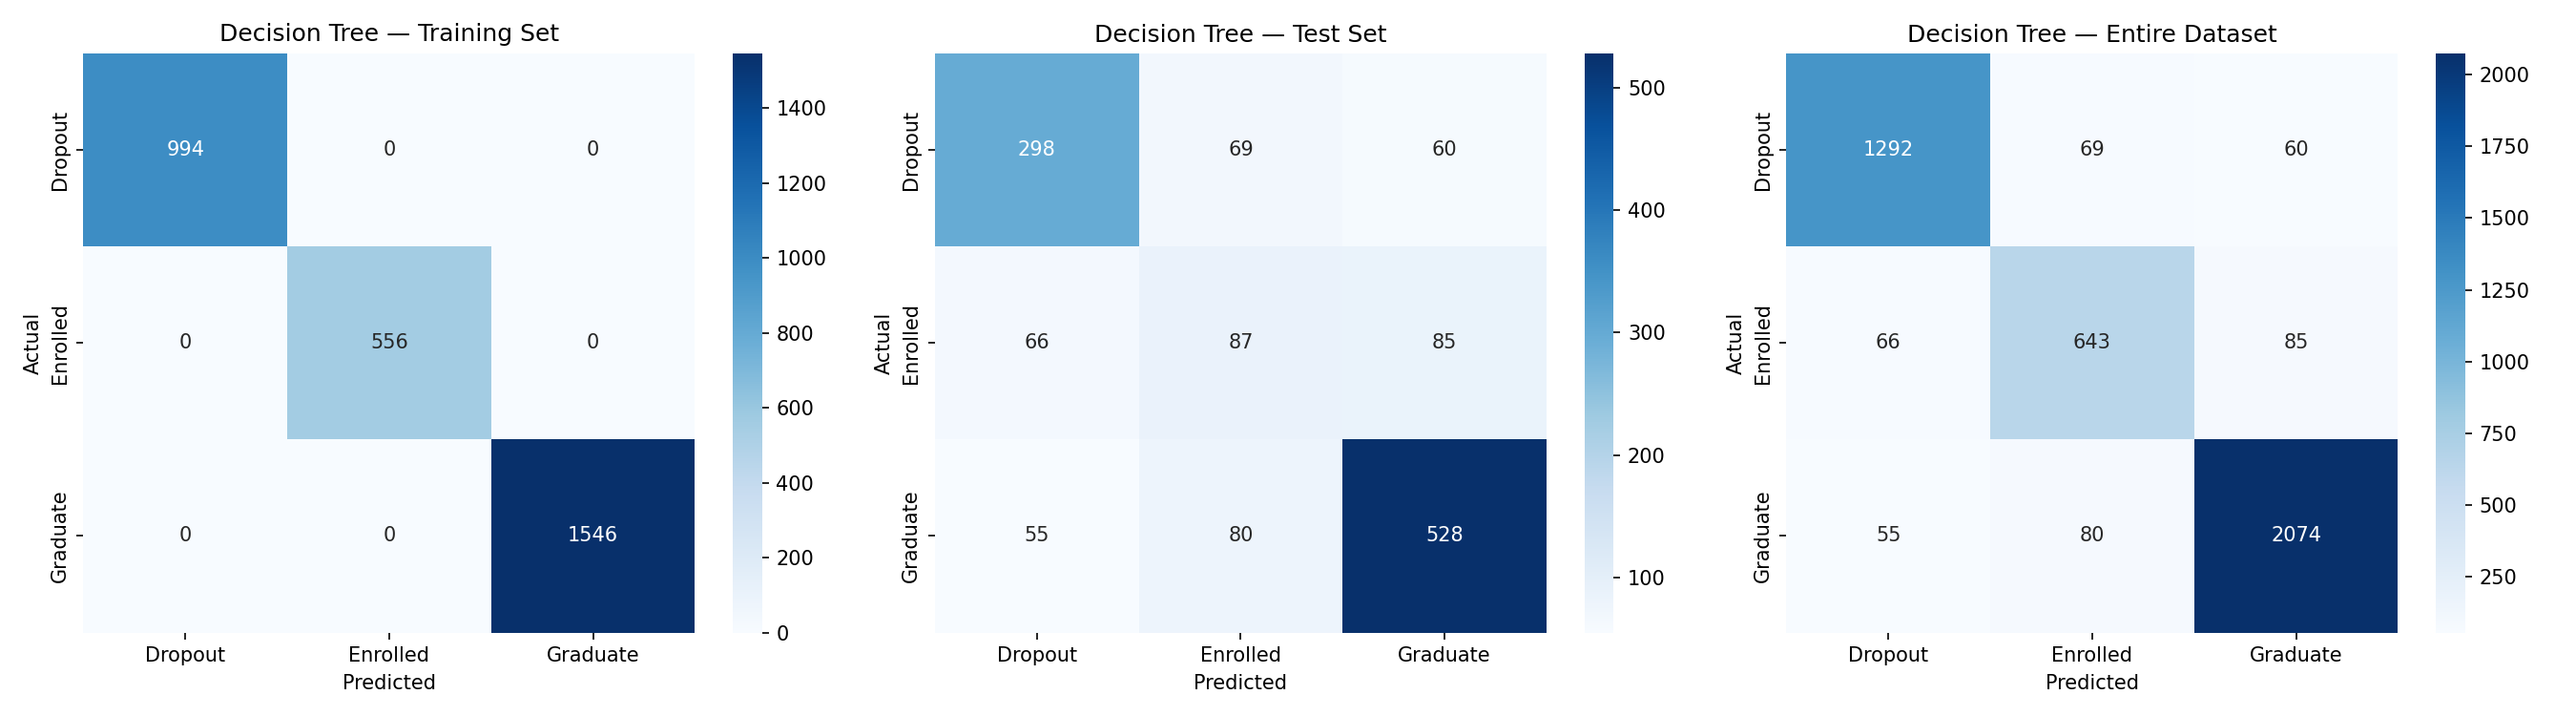
\includegraphics[width=\linewidth]{confusion_matrix_dt.png}
  \caption{Decision Tree confusion matrices (train, test, entire).
    The test-set matrix shows heavy Dropout$\leftrightarrow$Enrolled
    and Enrolled$\to$Graduate confusions.}
  \label{fig:cm-dt}
\end{figure}

\begin{figure}[h]
  \centering
  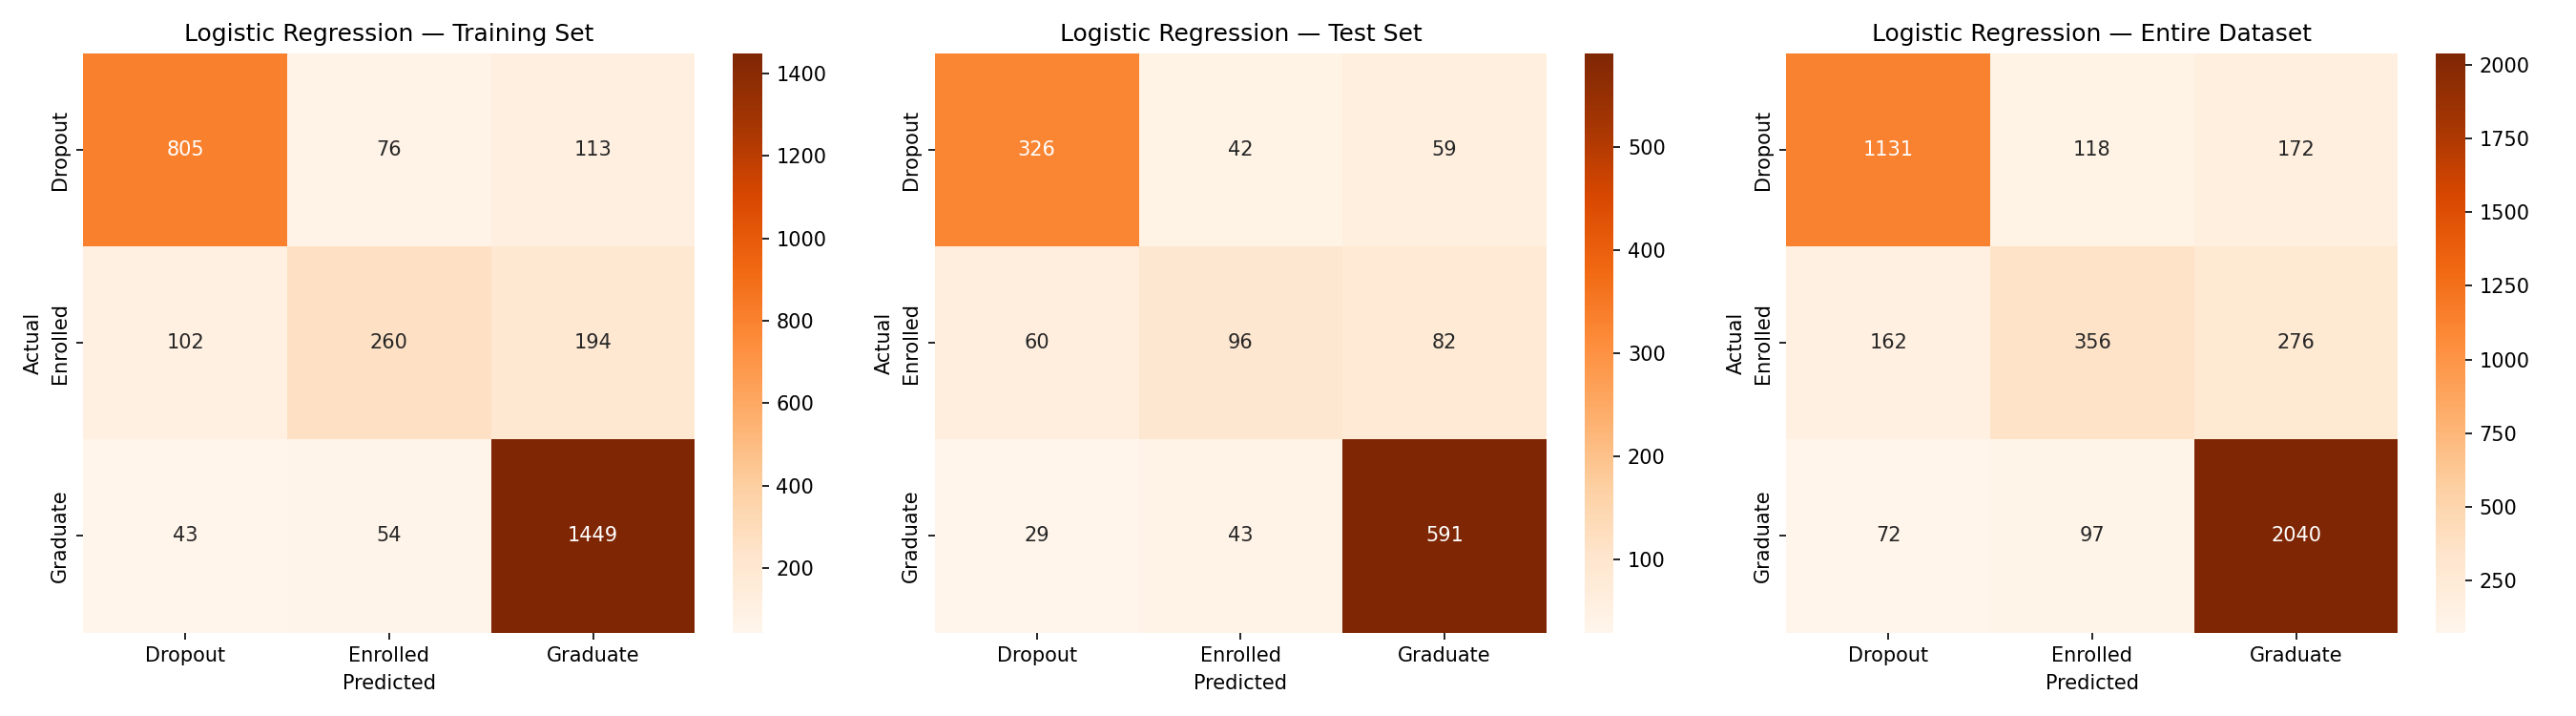
\includegraphics[width=\linewidth]{confusion_matrix_lr.png}
  \caption{Logistic Regression confusion matrices. LR concentrates
    Enrolled-class errors into the Graduate column (a more
    "reasonable" error than the Decision Tree's scatter).}
  \label{fig:cm-lr}
\end{figure}

\paragraph{Interpretation.} Enrolled is the hardest class for both
models (per-class F1 $\approx 0.37$ for DT, $0.46$ for LR). This
matches the t-SNE observation: currently-enrolled students occupy an
overlapping region between Dropout and Graduate. LR outperforms the
Decision Tree on every balanced metric; the Decision Tree's
$1.000$ training accuracy with only $0.688$ on test is a textbook
overfitting signal that we address via pruning and class-weighting
in Section~\ref{sec:eval}.

\subsection{Evaluation and Choice of Prediction Model}
\label{sec:eval}
% Aim: ~1.5 pages. Full metrics + ROC + validation strategies.

\paragraph{Metrics.} We compute accuracy, precision, recall, and F1
(macro and weighted) from the test confusion matrices, and OvR
multiclass ROC/AUC using predicted probabilities.

\begin{table}[h]
  \centering
  \caption{Baseline test-set metrics. LR dominates on every
    class-balanced criterion.}
  \label{tab:metrics}
  \begin{tabular}{lrrrrr}
    \toprule
    Model & Accuracy & Precision\,\textsubscript{macro} & Recall\,\textsubscript{macro} & F1\,\textsubscript{macro} & AUC\,\textsubscript{macro} \\
    \midrule
    Decision Tree       & $0.688$ & $0.621$ & $0.620$ & $0.621$ & $0.729$ \\
    Logistic Regression & $0.764$ & $0.711$ & $0.689$ & $0.696$ & $0.862$ \\
    \bottomrule
  \end{tabular}
\end{table}

\paragraph{Validation-driven improvement.} We compare two strategies
on the training split only:
\begin{itemize}
  \item \textbf{CV (GridSearchCV)} with 5-fold
        \texttt{StratifiedKFold(shuffle=True, random\_state=42)},
        scoring \texttt{f1\_macro}.
  \item \textbf{Holdout validation}: $80/20$ split of the training
        fold; hyperparameters chosen on the validation fold; final
        model refit on the full training fold.
\end{itemize}

Both strategies prefer Decision Tree \texttt{max\_depth=5} with
\texttt{class\_weight="balanced"}, and Logistic Regression
$C{=}1.0$ with \texttt{class\_weight="balanced"}. Tuning lifts the
Decision Tree's macro AUC from $0.729$ to $0.838$ --- the biggest
improvement in the project, directly addressing the overfitting
observed in Section~2.4. LR gains are marginal because the baseline
is already well-regularised.

\paragraph{Further discussion (100--200 words).}
On the fixed 70/30 test split, Logistic Regression outperforms the
Decision Tree on class-balanced metrics. Baseline LR reaches
macro-F1 $\approx 0.70$ and macro AUC $\approx 0.86$, while the
unconstrained DT sits at macro-F1 $\approx 0.62$ and macro AUC
$\approx 0.73$ --- consistent with higher variance and overfitting
risk in the tree. ROC/AUC analysis confirms the ordering, and the
\emph{Enrolled} class has the lowest one-vs-rest AUC across every
model, matching the confusion-matrix pattern where Enrolled is most
often predicted as Graduate. We improved both models via
validation without ever touching the test set. CV and holdout
tuning select similar LR settings and test performance barely
changes, suggesting LR is already near a good optimum under this
feature representation. For the Decision Tree, tuning (depth cap
plus class weighting) lifts macro AUC from $0.73$ to $0.84$ and
narrows the gap to LR. We select the CV-tuned LR as the final
operating model on macro-F1/AUC held-out performance.

% =====================================================================
\section{Open-ended Exploration}
% Aim: 1--1.5 pages. Pending PRs #10 and #11.

\textbf{[PHASE 6 — fill in once PRs \#10 and \#11 land.]}

\subsection{Feature Engineering (PR \#11)}
% Narcissa2005: business-driven features + pipelines
% TODO: summarise the feature set (e.g. "approval ratio",
% "tuition-paid flag interaction") and report the honest CV gain
% after the Pipeline fix.

\subsection{Additional Model Comparison (PR \#10)}
% ymyymy-666: Phase 6 scope to be expanded beyond DT/LR tuning
% TODO: compare $\geq 3$ model classes using cross-validation
% (e.g. SVM, Random Forest, Gradient Boosting); report macro-F1
% and macro AUC; identify the best model and rationalise the
% choice.

% =====================================================================
\section{Conclusion}
% Aim: ~0.5 page.

We built an end-to-end supervised learning pipeline for a $4{,}424$-sample,
three-class student-outcome problem. The Enrolled class is inherently
harder than Dropout and Graduate --- a finding consistent across
t-SNE visualisation, clustering analysis, and every classifier we
trained. Logistic Regression with standardised features and balanced
class weights is our recommended operating model
(test macro-F1 $\approx 0.69$, macro AUC $\approx 0.86$). The
Decision Tree, while initially overfitting, is a useful interpretable
backup once constrained to \texttt{max\_depth=5}.
\textbf{[Phase 6: one-sentence summary of the best open-ended
finding.]} Practically, the Enrolled prediction gap suggests the
dataset would benefit from time-to-event framing (survival analysis)
rather than static three-class classification --- a direction we
flag for future work.

% =====================================================================
\section*{References}
% ~0.5 page; not counted toward the 5--10 page limit.

\begin{thebibliography}{9}
  \bibitem{uci_dropout}
    M.~V.~Martins, D.~Tolledo, J.~Machado, L.~M.~T.~Baptista,
    and V.~Realinho. ``Predict Students' Dropout and Academic
    Success.'' UCI Machine Learning Repository, 2021.
  \bibitem{sklearn}
    F.~Pedregosa et al. ``Scikit-learn: Machine Learning in Python.''
    \emph{Journal of Machine Learning Research}, 12:2825--2830, 2011.
  \bibitem{vandermaaten_tsne}
    L.~van der Maaten and G.~Hinton. ``Visualizing Data using
    t-SNE.'' \emph{Journal of Machine Learning Research},
    9:2579--2605, 2008.
  % Add further citations as needed.
\end{thebibliography}

\section*{Credit}
% Per PDF: contribution of each group member AND GenAI tools.

\paragraph{Group member contributions.}
\begin{itemize}
  \item \textbf{<Member 1>} --- Phase 1 (preprocessing) lead,
        report section~2.1.
  \item \textbf{<Member 2>} --- Phase 2 (t-SNE) lead, report
        section~2.2.
  \item \textbf{<Member 3>} --- Phase 3 (clustering) lead, report
        section~2.3.
  \item \textbf{<Member 4>} --- Phase 4 (prediction) lead, report
        section~2.4.
  \item \textbf{<Member 5>} --- Phase 5 (evaluation) lead, report
        section~2.5.
  \item Phase 6 work split between <Members> per PRs~\#10 and~\#11.
\end{itemize}

\paragraph{GenAI disclosure.}
Claude (Anthropic, Opus~4.x via Claude Code) was used for code
review and debugging support across Phases 3--5 (specifically:
identifying a cluster-indexing bug in Phase 3, flagging target
leakage in Phase 6 feature-engineering, suggesting the
\texttt{StandardScaler}/\texttt{Pipeline} fix in Phase 4, and
proposing refactors that were manually reviewed and committed).
Claude also assisted in drafting the structure of this report; all
numerical results, figures, and interpretations were produced and
verified by the authors. Estimated AI-assisted share of final report
writing: \textless\,$25\%$.

\end{document}
